% ============================================================================
% Paper A — Memory and chaos in a physics-constrained relaxation substrate
% Target: Chaos, Solitons & Fractals (Elsevier)
%
% COMPILATION: latexmk -pdf PAPER_A.tex   (or pdflatex x2)
%
% SUBMISSION NOTES:
%  - Elsevier "Your Paper Your Way": the current format is accepted for
%    submission; switch to elsarticle.cls (final, 3p/1p) at acceptance.
%  - This file compiles standalone with the standard article class.
% ============================================================================
\documentclass[11pt]{article}

\usepackage[margin=1in]{geometry}
\usepackage{amsmath,amssymb}
\usepackage{graphicx}
\usepackage{booktabs}
\usepackage{caption}
\usepackage[hidelinks]{hyperref}
\usepackage{microtype}

\graphicspath{{../figures/}}

\newcommand{\Dt}{\Delta t}
\newcommand{\MCI}{\mathrm{MC}}

\title{Memory and chaos in a physics-constrained relaxation substrate:
phase diagram, multi-timescale forgetting, and disturbance robustness}

\author{Yaming Hu\thanks{ORCID: 0009-0003-1406-0485. Independent
Researcher, Guiyang, Guizhou Province, China. E-mail:
\texttt{64687555@qq.com}.}}

\date{\today}

\begin{document}

\maketitle

\begin{abstract}
Reservoir computing exploits the fading-memory dynamics of a physical substrate,
yet the memory--chaos trade-off is usually studied on abstract recurrent networks
with hand-tuned leak rates. We characterize a physics-constrained relaxation
substrate inspired by Si$_3$N$_4$ shallow-trap charge storage: $N$ units with a
log-normal time-constant spectrum (median $\tau_0 \approx 174\,\mu$s,
CV $=0.20$) coupled through a per-pulse, topology-dependent modulation of the
injection coefficient. Sweeping the coupling strength $\kappa$ across five
topology families and measuring the finite-time Lyapunov exponent $\lambda$, the
held-out Jaeger memory capacity, and input separation, we find a sharp
order--chaos transition at $\kappa^\ast \in (25,30)$: the held-out memory
capacity peaks 24--53\% above the uncoupled baseline just before the
transition, and deep chaos destroys memory. The decay of linear memory follows
an analytically derived forgetting kernel $M(t)=\int p(\tau)e^{-t/\tau}\,d\tau$
over the log-normal trap spectrum (Pearson $r=0.97$ against the measured
memory-capacity curve). The $1/e$ horizon stays near
$\tau_0/\bar{\Delta t}\approx 16$ pulses as the spectrum widens (measured
12--16 pulses for CV $\in[0.02,1.0]$), while the width CV controls the tail
weight. Finally, a homeostatic regulator that
estimates $\lambda$ online and adjusts $\kappa$ to a near-critical target
improves post-disturbance held-out memory by 8--18\% under temperature drift,
edge damage, and readout noise.
\end{abstract}

\noindent\textbf{Keywords:} chaos; reservoir computing; memory capacity;
forgetting kernel; homeostasis; relaxation substrate; finite-time Lyapunov
exponent.

\section{Introduction}
\label{sec:intro}

Physical reservoir computing proposes that a complex dynamical substrate --- a
spiking neural microcircuit \cite{maass2002}, an optoelectronic system
\cite{larger2012}, a memristive array \cite{du2017}, or a charge-trap device
\cite{prior} --- can serve as a nonlinear, fading-memory kernel whose
instantaneous state is linearly read out by a trained network. The theoretical
foundations are well established: the fading-memory property dates to the
Volterra/Wiener system-identification literature \cite{boyd1985}, and echo
state networks \cite{jaeger2001} and
liquid state machines \cite{maass2002} rely on the \emph{echo state property}
(contracting, input-forgetting dynamics), and the \emph{edge of chaos}
maximizes the computational capability of driven recurrent systems
\cite{bertschinger2004}. Dambre et al.\ \cite{dambre2012} formalized the total
information-processing capacity of dynamical systems, showing a universal
trade-off between linear memory and nonlinear processing. On the memory side,
multi-timescale synaptic models \cite{fusi2005,benna2016} show that memory
retention is dramatically extended by a \emph{spectrum} of time constants:
cascade models achieve near power-law forgetting from many exponentially
decaying components.

For a physical reservoir, the time-constant spectrum is not a free
hyperparameter --- it is a \emph{material property}. Shallow-trap charge storage
in Si$_3$N$_4$ exhibits thermally activated relaxation with a log-normal spread
of trap time constants; our prior work \cite{prior} established that this
substrate encodes pulse-interval patterns through exponential relaxation with
$\tau_0 \approx 174\,\mu$s at 300~K and a device-to-device spread of CV $=0.20$,
achieving 79.6\% four-class hybrid encoding accuracy in a purely numerical
(Digital-Model) setting. That work, however, treated the substrate as a
\emph{parallel} array of independent devices; the coupling between devices ---
the element that could push the substrate toward richer, near-critical dynamics
--- was only implemented as a quasi-static modulation of the effective injection
coefficient across blocks.

This paper closes that gap. We introduce the \emph{per-pulse temporal
generalization} of the topology coupling: every pulse, each unit's injection
coefficient is modulated by a topology-dependent contrast against its
neighbors' current ratios, making the substrate a genuinely recurrent, tunable
dynamical system with a physical chaos knob $\kappa$. Our contributions are:
\begin{enumerate}
\item \textbf{A memory--chaos phase diagram} for a physics-constrained
relaxation substrate: the finite-time Lyapunov exponent $\lambda$, the held-out
Jaeger memory capacity, and the input separation, all as functions of the
coupling strength $\kappa$, across five topology families (bidirectional ring,
unidirectional ring, hub-and-spoke, lateral-inhibition ring, random graph) and
two coupling sign conventions (negative- and positive-feedback contrast), with
an additive state-coupling control.
\item \textbf{An analytic forgetting kernel} $M(t)=\int p(\tau)e^{-t/\tau}
\,d\tau$ for the log-normal trap spectrum, validated against the measured
memory-capacity curve (Pearson $r=0.97$), which turns the device-physics spread
CV into a \emph{design knob for the forgetting curve}.
\item \textbf{A homeostatic chaos regulator} that estimates $\lambda$ online
from Benettin twin trajectories and adjusts $\kappa$ to a near-critical target,
restoring 8--18\% of held-out memory after environmental disturbances
(temperature drift, edge damage, readout noise) where fixed coupling cannot.
\end{enumerate}

Throughout, we use a \emph{held-out} memory-capacity protocol: ridge fits are
trained on the first 70\% of a driving stream and evaluated on the last 30\%
(with a $k_{\max}$-length leakage buffer). We show that the common in-sample
Jaeger convention dramatically overstates memory in the chaotic regime, which
is a methodological caution for the field.

\section{Substrate model}
\label{sec:model}

\subsection{Single-unit relaxation}

Each unit models a Si$_3$N$_4$ shallow-trap population with effective trap
occupancy $x_i \in [0,1]$. A write pulse of width $p_w=1\,\mu$s injects charge
with coefficient $\alpha$; the occupancy then relaxes exponentially with the
unit's trap time constant $\tau_i$ both during the pulse width and during the
inter-pulse interval $\Dt_t$. The per-pulse update is
\begin{equation}
x_i(t+1) = \Big[x_i(t) + \alpha_{\mathrm{eff},i}(t)\big(1-x_i(t)\big)\Big]\,
e^{-p_w/\tau_i} e^{-\Dt_t/\tau_i}, \qquad x_i \in [0,1],
\label{eq:update}
\end{equation}
and the observable current ratio is $i_i = e^{\gamma x_i}$ with
$\gamma=\ln 100$ (a 100:1 ON/OFF ratio at $I_{\mathrm{HRS}}=50$~fA). The trap
time constants are drawn from a log-normal distribution with median
$\tau_0=174\,\mu$s (from $E_a=0.55$~eV, $\nu=10^{13}$~s$^{-1}$, $T=300$~K) and
CV $=0.20$: $\tau_i \sim \mathrm{Lognormal}(\mu,\sigma)$ with
$\sigma^2=\ln(1+\mathrm{CV}^2)$; the log-normal form follows from a Gaussian
spread of activation energies (Appendix~\ref{app:spectrum}).

\subsection{Per-pulse topology coupling}

The injection coefficient of unit $i$ at pulse $t$ is modulated by a
topology-dependent contrast between its own current ratio and a weighted mean
of its neighbors' current ratios:
\begin{equation}
\alpha_{\mathrm{eff},i}(t) = \mathrm{clip}\Big(\alpha_0\big(1 + \kappa\,
g_i(t)\big),\, \alpha_{\min}, \alpha_{\max}\Big),
\label{eq:coupling}
\end{equation}
with two contrast conventions --- \emph{negative feedback} (mode 1):
$g_i=(\bar{i}_{\mathcal{N}(i)} - i_i)/i_i$; and \emph{positive feedback}
(mode 2): $g_i = (i_i - \bar{i}_{\mathcal{N}(i)})/\bar{i}_{\mathcal{N}(i)}$ ---
where $\bar{i}_{\mathcal{N}(i)}$ is the weighted mean of neighbor current
ratios (row-normalized weights). The base injection coefficient is
$\alpha_0=0.02$; the physical clip range
$[\alpha_{\min},\alpha_{\max}]=[0.001,0.10]$ bounds the injection coefficient.
A control condition replaces the contrast coupling with an additive state drive
$x_i \mathrel{+}= \kappa\,\bar{x}_{\mathcal{N}(i)}$ after the standard update
(the non-physical, ``textbook ESN'' style). All coupling is computed two-pass
(contrasts from the pre-update state, then all units updated), making the step
order-independent (Appendix~\ref{app:update}). At $\kappa=0$ the model reduces exactly to
the parallel array of \cite{prior} (verified to machine precision).

Five topologies over the $N=256$ units are used: \textbf{ring\_bidir} (each
unit watches its two neighbors), \textbf{ring\_unidir} (each unit watches its
predecessor), \textbf{hub\_star} (satellites watch a fixed hub),
\textbf{lateral\_ring} (distance-decayed neighbors within radius 4), and
\textbf{random\_graph} (Erd\H{o}s--R\'enyi, mean degree 8, fixed structure
across the sweep). The drive is an i.i.d.\ uniform interval stream
$\Dt_t \sim U[2,20]\,\mu$s, the fast-drive regime in which the nominal memory
window is $N_{\mathrm{eff}} = \tau_0/\bar{\Dt} \approx 16$ pulses.

\section{Characterization methods}
\label{sec:methods}

\textbf{Finite-time Lyapunov exponent.} For a driven system the relevant
quantity is sensitivity to initial conditions under identical drive. We evolve
a twin trajectory perturbed by $\epsilon=10^{-8}$ per unit, renormalize the
separation to $\epsilon\sqrt{N}$ every 10 pulses (Benettin scheme), and report
$\lambda = \langle \ln(d/\epsilon\sqrt{N})\rangle$ per pulse, averaged over
the full stream (detailed iteration steps in Appendix~\ref{app:benettin}).

\textbf{Held-out memory capacity.} Following Jaeger, the linear memory of lag
$k$ is the squared Pearson correlation between the ridge-decoded value of the
driving interval $\Dt_{t-k}$ and its true value, decoded from the current-ratio
observables at time $t$. We fit the ridge readout (regularization
$\lambda_r=1$, features standardized with training-segment statistics) on the
first 70\% of the collected stream, hold out a $k_{\max}=50$-step leakage
buffer, and evaluate on the last 30\%; $\MCI_{\mathrm{total}} = \sum_{k=1}^{50}
r_k^2$. The held-out protocol is essential: the in-sample convention inflates
memory in the chaotic regime by 7--19$\times$ relative to held-out
evaluation (Section~\ref{sec:chaos}). The
estimator derivation and the linear-reservoir closed form that anchors the
theory are given in Appendix~\ref{app:mc}.

\textbf{Input separation.} The RMS distance between the state trajectories
produced by two different i.i.d.\ drives from the same initial condition,
averaged over the collected window --- a proxy for how far different input
histories push the state.

\textbf{Activity proxy.} The running standard deviation of the population-mean
current ratio over a 200-pulse window (used in the homeostat analysis).

\section{Phase diagram}
\label{sec:phasediagram}

All quantities below are means over 10 independent seeds (paired $\tau$ draws
across $\kappa$); the full table is in Supplementary Table~S1
(data/substrate\_phase\_diagram\_v2.csv). Table~\ref{tab:phase} summarizes the
per-topology behavior.

\begin{table}[t]
\centering
\caption{Per-topology summary of the $\kappa$ sweep (held-out MC, 10 seeds).
Peak gains are relative to the uncoupled baseline MC $=9.07$.
}\label{tab:phase}
\begin{tabular}{@{}llp{6.2cm}p{3.4cm}@{}}
\toprule
Topology & Mode & Transition / behavior & Peak MC (vs.\ 9.07) \\
\midrule
ring\_bidir      & negative & order--chaos at $\kappa^\ast\in(25,30)$ & 11.88 ($+30\%$) at $\kappa=20$ \\
lateral\_ring    & negative & order--chaos at $\kappa^\ast\in(25,30)$ & 11.29 ($+24\%$) at $\kappa=20$ \\
random\_graph    & negative & order--chaos at $\kappa^\ast\in(25,30)$ & 13.91 ($+53\%$) at $\kappa=25$ \\
ring\_unidir     & positive & self-limited criticality ($\lambda\approx-0.002$), $\kappa\in[1,5]$ & 0.12--0.39$^{\ast}$ \\
hub\_star        & positive & frozen (clip fraction 1.0) & none \\
\bottomrule
\end{tabular}

\medskip
\footnotesize{$^{\ast}$no held-out linear memory (in-sample MC 18--20).}
\end{table}

\subsection{Negative-feedback family: stabilization then a sharp transition}
\label{sec:negfb}

For the mode-1 (negative-feedback) topologies, weak-to-moderate coupling
\emph{stabilizes}: $\lambda$ becomes more negative ($-0.065 \to -0.090$ as
$\kappa$ grows to 10 for the ring) and the mean absolute contrast $|g|$
shrinks ($0.15 \to 0.01$), i.e., the coupling actively homogenizes neighboring
states. Memory rises modestly in this regime (ring\_bidir held-out MC
$9.1 \to 10.6$ at $\kappa=10$). At $\kappa \in (25, 30)$ the system crosses a
sharp order--chaos transition ($\lambda$ jumps from $\approx -0.05$ to $>0$)
for all three mode-1 topologies; the transition is accompanied by the onset of
$\alpha_{\mathrm{eff}}$ clipping (clip fraction 0.3--0.6), i.e., the physical
bounds start to bind. \textbf{The held-out memory capacity peaks in the last
ordered configuration before the transition}: random\_graph at $\kappa=25$
reaches MC $=13.91$ vs.\ $9.07$ uncoupled ($+53\%$), ring\_bidir at $\kappa=20$
$+30\%$, lateral\_ring at $\kappa=20$ $+24\%$.

\subsection{Transition mechanism: coupling versus the physical clip}
\label{sec:clipablation}

The sharp transition at $\kappa^\ast$ coincides with the onset of
$\alpha_{\mathrm{eff}}$ clipping (clip fraction 0.3--0.6), which raises
the question of whether the chaos is produced by the topology coupling
or by the physical bounds. A follow-up sweep (data/s27\_clip\_kappa
\_fine\_v1.csv; $\kappa\in[20,30]$ at unit resolution $\times$
$\alpha_{\max}\in\{0.1,0.2,0.5\}$, 10 seeds) answers it. First, the fine
grid pins the mean-FTLE crossing at $\kappa^\ast = 25.3$ (lateral\_ring),
27.4 (ring\_bidir), and 27.9 (random\_graph), all inside the $(25,30)$
bracket above --- the transition is sharp at unit resolution, not a grid
artifact. Second,
widening the clip five-fold ($\alpha_{\max}=0.5$) does not move the
transition for the two topologies with the largest memory gains:
$\kappa^\ast = 25.3\to25.4$ (lateral\_ring; shift $+0.05$) and
$27.9\to27.7$ (random\_graph; shift $-0.21$). The order--chaos transition
is therefore
\emph{coupling-driven}: the clip is a consequence of the large contrasts
it bounds, not their cause. ring\_bidir is the one exception --- its
crossing moves $+3.4$ under the wider clip, so the
bound contributes to that topology's transition onset. A secondary
result: widening the clip raises the ring\_bidir memory peak from 11.9
to 17.7 ($\alpha_{\max}=0.2$), showing that for ring-like topologies the
physical clip currently caps held-out memory --- a fabrication-tunable
trade.

\subsection{Positive-feedback family: self-limited criticality, separation without linear memory}

The mode-2 (positive-feedback) topologies behave very differently. The
\textbf{unidirectional ring} self-limits at criticality: $\lambda$ approaches
$\approx -0.002$ (within our FTLE resolution of zero) over a half-decade of
coupling strength $\kappa\in[1,5]$, held there by the $\alpha_{\mathrm{eff}}$
clip (clip fraction 0.5--1.0) interacting with the $(1-x)$ saturation;
beyond $\kappa=5$ the ordered regime reasserts itself
($\lambda\approx-0.026$ at $\kappa=10$). This
regime shows the \emph{largest} input separation of the entire study
(inter-stream RMS 0.054--0.085 vs.\ 0.022 baseline) but \emph{zero} held-out
linear memory (MC $0.12$--$0.39$, despite in-sample MC of 18--20). The
exponential current nonlinearity makes the saturated critical states
information-rich but linearly undecodable --- a clean demonstration of the
separation--memory trade-off: separation-rich critical states require nonlinear
readout to be exploited. The \textbf{hub-and-spoke} topology freezes instead:
with no feedback loop through the hub, satellites saturate into bistable
above/below-hub states (clip fraction 1.0) and memory never exceeds the
baseline.

\subsection{Chaos destroys memory; in-sample MC is misleading}
\label{sec:chaos}

In the chaotic regime ($\kappa=50,100$), the held-out MC collapses to 1.85--4.4
(a 3--7$\times$ drop from the peak) --- a sharp contrast to the successful
reservoir prediction of externally driven chaotic systems \cite{pathak2018},
where the drive, not the internal dynamics, supplies the input trace. The in-sample (train-segment) MC, by
contrast, \emph{explodes} to 30--35 --- an overfitting artifact of ridge
decoding the huge-amplitude chaotic state; the held-out protocol reveals the
true destruction of memory. We therefore report held-out MC throughout and
recommend the practice to the field.

\subsection{The additive control: why physics constraints matter}

The additive state-coupling control (mode 3, textbook ESN style) reaches its
best in-sample MC (17--22) near its saturation threshold
($\kappa\approx 0.08$--0.1) and then dies: the state pins at the saturation
boundary and the FTLE estimate collapses numerically (a signature of degenerate
dynamics). Its held-out MC never exceeds the uncoupled baseline meaningfully
(max 9.1), and the operating window is a narrow band before saturation. The
physics-constrained contrast coupling, by contrast, remains well-behaved across
three decades of $\kappa$ and achieves the memory gains above --- the physical
clip acts as a built-in stability regulator.

\section{Multi-timescale forgetting theory}
\label{sec:kernel}

\subsection{The kernel}

The linear memory of a single trap for an input at lag $t$ decays as
$e^{-t/\tau}$. The substrate's population forgetting kernel is the average over
the log-normal spectrum:
\begin{equation}
M(t) = \int_0^\infty p(\tau)\, e^{-t/\tau}\, d\tau, \qquad
p(\tau)=\mathrm{Lognormal}(\tau_0,\mathrm{CV}).
\label{eq:kernel}
\end{equation}
We evaluate $M(t)$ by Gauss--Hermite quadrature (160 nodes, exact to machine
precision; derivation in Appendix~\ref{app:quadrature}). Three properties follow
(Fig.~\ref{fig:forgetting}):
\begin{enumerate}
\item \textbf{The $1/e$ horizon is median-pinned.} $M(\tau_0/\bar{\Dt})
\approx e^{-1}$ --- within a few percent for CV $\le 0.5$ and within
$\sim$25\% at CV $=1.0$; the horizon is 12--16 pulses for CV
$\in[0.02,1.0]$, in agreement with the nominal window $N_{\mathrm{eff}}\approx
16$. The \emph{median} time constant sets where memory is; the width sets how
it decays.
\item \textbf{The tail steepens with narrowing spectrum.} The log-log slope
$d\ln M/d\ln t$ at long lags is $-60.6$ at CV $=0.2$ and rises to $-7.1$ at
CV $=1.0$ (and $-\infty$ in the CV$\to0$ single-exponential limit). A wider
trap spread yields a heavier tail --- slower forgetting of old information.
\item \textbf{Comparison to cascade ideals.} The log-Gaussian tail
$\ln M(t)\sim -(\ln t-\mu)^2/(2\sigma^2)$ is \emph{slower} than a single
exponential but \emph{steeper} than the near power-law retention of
multi-timescale cascade models \cite{fusi2005,benna2016}. Reaching
power-law-like retention would require an unrealistically wide spectrum; the
physical substrate therefore occupies a specific point in the forgetting design
space set by CV.
\end{enumerate}

\subsection{Validation against the measured memory capacity}

The measured parallel-substrate curve $\sqrt{\MCI(k)}$ (held-out) tracks
$M(k\cdot\bar{\Dt})$ at CV $=0.20$ with \textbf{Pearson $r=0.97$}
(data/forgetting\_curve\_theory\_overlay\_v1.json); at lag 10
the two agree almost exactly (0.520 vs.\ 0.523), with systematic damping at
short lags (readout regression attenuation for a random drive). The
device-physics spectrum thus predicts the substrate's empirical memory curve
from first principles.

\textbf{Implication.} CV --- a fabrication-controllable spread parameter --- is
a \emph{design knob for the forgetting curve}. This is the quantitative basis
for the ``physics as a structured state-space kernel'' view: the substrate
realizes a specific multi-timescale kernel with a tunable tail.

\textbf{The coupled-substrate caveat (task-level CV sweep).} The kernel theory
is single-unit; at the task level the CV knob's direction is
operating-regime-dependent --- uncoupled operation follows the theory (wider
CV, heavier tail, more retained memory), while coupled near-critical operation
prefers narrow spectra. The full sweep (CV $\in\{0.1,0.2,0.4\}$ $\times$
\{uncoupled, random\_graph $\kappa=25$, ring\_bidir $\kappa=20$\}, 10 seeds) is
given in Supplementary Note~1 (Fig.~S1); the kernel-level stability across
CV $\in[0.02,1.0]$ is in Fig.~\ref{fig:forgetting} and
Appendix~\ref{app:quadrature}.

\textbf{The kernel survives coupling (shape stability).} The single-unit
theory was validated on the parallel substrate; the committed per-lag
memory curves let us ask whether the coupled substrate's curve is still
kernel-shaped. The \emph{physical} spectrum $(174\,\mu$s, CV $0.20)$
achieves Pearson $r = 0.91$--$0.99$ against $\sqrt{\mathrm{MC}(k)}$ over
$\kappa \in \{15,\dots,30\}$ of all three mode-1 topologies ($r=0.98$ at
random\_graph $\kappa{=}25$), without any re-fitting
(data/kernel\_coupling\_shape\_v1.json; quadrature as in
Appendix~\ref{app:quadrature}): the kernel shape survives coupling. The
approach to the transition dilates the memory kernel (consistent with
the near-critical slowdown of Section~\ref{sec:negfb}), but single
curves cannot separate an effective-median shift from a width change
(the fit saturates at wide CV), so we report the shape stability
quantitatively and the dilation qualitatively rather than as a precise
renormalization map.

\section{Disturbance robustness and the \texorpdfstring{$\lambda$}{lambda}-homeostat}
\label{sec:homeostat}

\subsection{The disturbed memory landscape}

We subject the random-graph substrate ($\kappa=25$, the nominal optimum) to
three abrupt disturbances at $t=10$k in an online Mackey--Glass forecasting
task (RLS readout): \textbf{temperature drift} (all $\tau$ scaled by 1.5),
\textbf{edge damage} (40\% of coupling edges removed), and \textbf{readout
noise} ($\sigma=0.1\times$ feature std). The held-out MC--$\kappa$ landscape
shifts with the disturbance: noise reduces memory everywhere (peak 10.05 vs.\
13.98 nominal), edge damage \emph{improves} memory (16.53 --- removing
homogenizing edges), and temperature drift flattens the landscape, retaining
substantial memory at larger $\kappa$ (11.01 at $\kappa=40$ vs.\ 6.95 nominal).
Consequently, any regulator anchored to a \emph{fixed activity
target} (a common homeostatic design) fails: the target's optimum is not
disturbance-invariant (this negative design result motivated the
$\lambda$-homeostat).

\subsection{The \texorpdfstring{$\lambda$}{lambda}-homeostat}

The homeostat estimates $\lambda$ directly: every 1000 pulses it runs a
400-pulse Benettin pair at the current $\kappa$ (40\% computational overhead)
and steps
\begin{equation}
\kappa \leftarrow \mathrm{clip}\big(\kappa + \eta\,\mathrm{clip}
(\lambda_{\mathrm{target}} - \hat\lambda,\, -1, 1),\, [1,60]\big),
\qquad \lambda_{\mathrm{target}} = -0.02, \quad \eta = 3,
\label{eq:homeostat}
\end{equation}
the slightly-ordered side of the transition where held-out MC peaks
(Section~\ref{sec:negfb}). The regulated system settles at $\kappa \approx
26$--27 under all conditions and achieves post-disturbance held-out MC gains of
$+7.6\%$ (none), $+18\%$ ($\tau$-drift), $+7.9\%$ (edge-prune), $+11.8\%$
(noise) over the fixed coupling (Table~\ref{tab:homeostat}), at broadly
comparable task-level NMSE (regulated up to $2\times$ worse on the gain arms,
better under readout noise; the RLS readout absorbs task-level differences,
and the substrate-level memory improvement is revealed by the
readout-independent MC probe). The
$\lambda$-homeostat is disturbance-type-agnostic because it tracks the
dynamical quantity itself rather than a proxy whose optimum shifts.
The estimate is also robust to its own noise: injecting Gaussian error
of up to $\sigma_\lambda = 0.10$ (the typical estimate magnitude is
$0.05$--$0.1$) into every Benettin estimate leaves the settled coupling
essentially unchanged (r3 $\kappa$ 28.5--28.7) and the post-disturbance
r3 MC within $0.16$ of the noiseless value with no significant paired
difference at any noise level (data/s32\_ftle\_noise\_v1.csv) --- the
clipped proportional feedback integrates over the estimation error.
A systematic $\lambda_{\mathrm{target}}$ sweep
($\lambda_{\mathrm{target}}\in\{-0.05,-0.02,-0.005,0\}\times\mathrm{CV}\in\{0.1,0.2,0.4\}$,
5 seeds; companion Paper~B, Table~2) identifies $\lambda_{\mathrm{target}}{=}0$
(the edge of chaos) as optimal: post-disturbance MC peaks near the edge of
chaos at every tested CV ($\lambda_{\mathrm{target}}{=}0$ optimal at CV=0.1 and 0.4;
the $-0.005$ setting marginally ahead at CV=0.2), with gains of $+25\%$
(CV=0.1), $+19\%$ (CV=0.2), $+5\%$ (CV=0.4) over fixed coupling --- updating
the manually tuned $-0.02$ used in the main results.

\begin{table}[t]
\centering
\caption{Post-disturbance held-out MC gains of the $\lambda$-homeostat over
fixed coupling (random\_graph substrate, Mackey--Glass online task, 10 seeds).
}\label{tab:homeostat}
\begin{tabular}{lcc}
\toprule
Disturbance & MC gain vs.\ fixed $\kappa$ & Settled $\kappa$ \\
\midrule
none         & $+7.6\%$ & 26--27 \\
$\tau$-drift & $+18\%$  & 26--27 \\
edge-prune   & $+7.9\%$ & 26--27 \\
readout noise & $+11.8\%$ & 26--27 \\
\bottomrule
\end{tabular}
\end{table}

\section{Discussion}
\label{sec:discussion}

\textbf{The physical parameter range bounds the accessible computation.} Three
material/design quantities jointly define the substrate's computational
envelope: the clip range $[\alpha_{\min},\alpha_{\max}]$ (which bounds coupling
and, in the positive-feedback family, self-limits the system at criticality),
the coupling threshold $\kappa^\ast$ (which separates the memory-rich ordered
side from the memory-destructive chaotic side), and the trap spectrum (which
fixes both the $1/e$ memory horizon and the forgetting tail). A clip-ablation
sweep (Section~\ref{sec:clipablation}) shows that $\kappa^\ast$ is invariant
to a five-fold widening of the clip for the memory-relevant topologies, so the
threshold is a genuine property of the coupling dynamics rather than a clip
artifact; the clip's role is secondary and topology-dependent. For the
neuromorphic-design question of what this device can compute, the answer
is a bounded but substantial region of the memory--chaos plane, fully
characterized here.

\textbf{Separation without linear memory.} The positive-feedback family reaches
true criticality ($|\lambda|\approx0$) with maximal separation yet zero held-out
linear memory. This is a caution for the common practice of tuning reservoirs to
the edge of chaos: at criticality the \emph{linear} readout loses the input
trace, and the separation must be exploited nonlinearly (a companion work
develops structure plasticity from functional connectivity). For linear readouts, the
optimal operating point is the \emph{last ordered configuration before the
transition} --- a slightly-subcritical target ($\kappa = 20$--25,
$\lambda \approx -0.05$), consistent with where the homeostat parks the
system ($\kappa \approx 26$--27).

\textbf{The forgetting kernel as design language.} $M(t)$ connects device
physics to the state-space-model literature: the substrate is a
hardware-realizable structured state-space kernel whose decay spectrum is set
by fabrication (CV). The $r=0.97$ validation shows the connection is
quantitative, not metaphorical.

\textbf{Spectrum knobs: location versus width.} Across the companion
papers three single-parameter spectrum knobs appear --- the material
CV here, the algorithmic EMA timescale $\tau_m$ (companion~C), and the
log-uniform coverage range of the state-space host (companion~D). They
are not interchangeable, and the distinction is quantitative: for a
log-normal spectrum the $1/e$ horizon is set by the \emph{location}
(median $\tau_0$: $M(\tau_0)\approx e^{-1}$ --- within a few percent for
CV $\le 0.5$, within $\sim$25\% at CV $=1.0$; measured
12--16 pulses over CV $\in[0.02,1.0]$) while the tail weight is set by
the \emph{width} (measured log-log slope $-60.6$ at CV $0.2$ vs.\ $-7.1$
at CV $1.0$). The companion's $\tau_m$ is a location knob (the
synthesized kernel's horizon scales with $\tau_m$, tail shape fixed),
and the log-uniform range is a width knob of a different family. The
practical corollary: specifying both a horizon and a tail requires two
independent knobs, and single-knob tuning moves exactly one observable
cross-section --- the same decomposition that makes the task-level CV
caveat above a re-projection onto a shifted location rather than a
contradiction (the effective median dilates under coupling,
Section~\ref{sec:kernel}).

\textbf{Limitations.} All results are numerical (Digital-Model level; no
fabricated device); the task-level CV sweep reveals an
operating-regime-dependent optimum (Supplementary Note~1); the homeostat's
gains are substrate-level (task-level NMSE is readout-compensated); FTLE
estimates are finite-time and resolution-limited near zero.

\section{Conclusion}
\label{sec:conclusion}

A physics-constrained relaxation substrate with per-pulse contrast coupling
possesses a well-defined memory--chaos phase diagram: negative-feedback
coupling buys 24--53\% more held-out memory up to a sharp transition,
positive-feedback coupling self-limits at criticality with maximal separation,
chaos destroys linear memory, and the log-normal trap spectrum fixes a
forgetting kernel that predicts the measured memory curve ($r=0.97$) with a
fabrication-tunable tail. A $\lambda$-homeostat restores 8--18\% of memory
after disturbances. These results turn a device-physics spread parameter into a
computational design knob and provide the substrate-level theory for the REDEM
online-learning architecture (companion paper \cite{companionB}).

\begin{figure}[t]
\centering
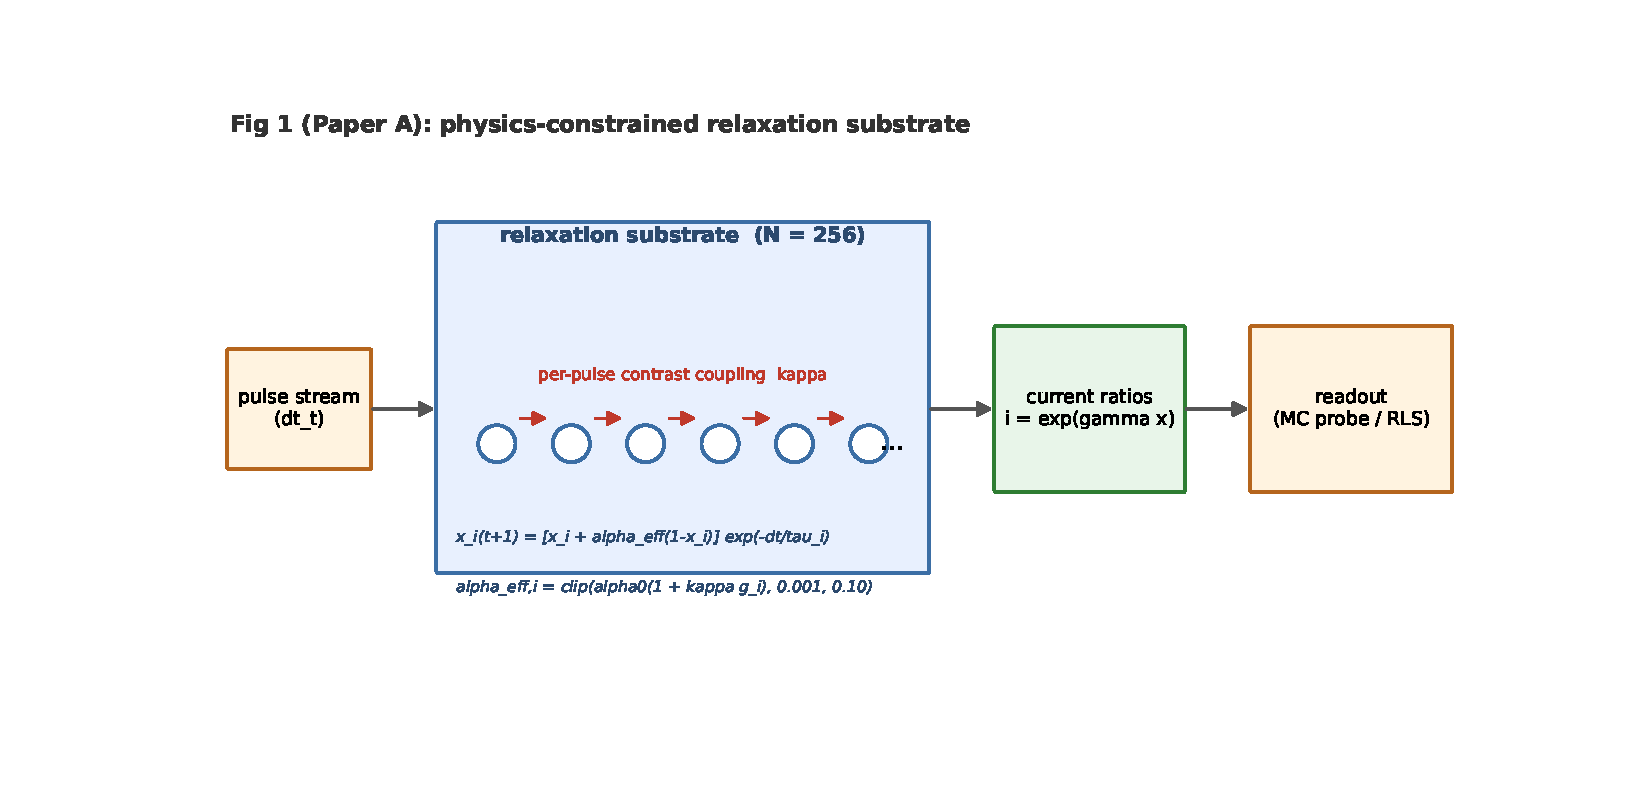
\includegraphics[width=0.92\textwidth]{paperA_fig1_substrate}
\caption{Substrate schematic (Paper A, Fig.~1): pulse stream, $N=256$
relaxation units with log-normal $\tau$ spectrum, per-pulse contrast coupling
(red arrows, $\kappa$), and the readout probe.}
\label{fig:schematicA}
\end{figure}

\begin{figure}[t]
\centering
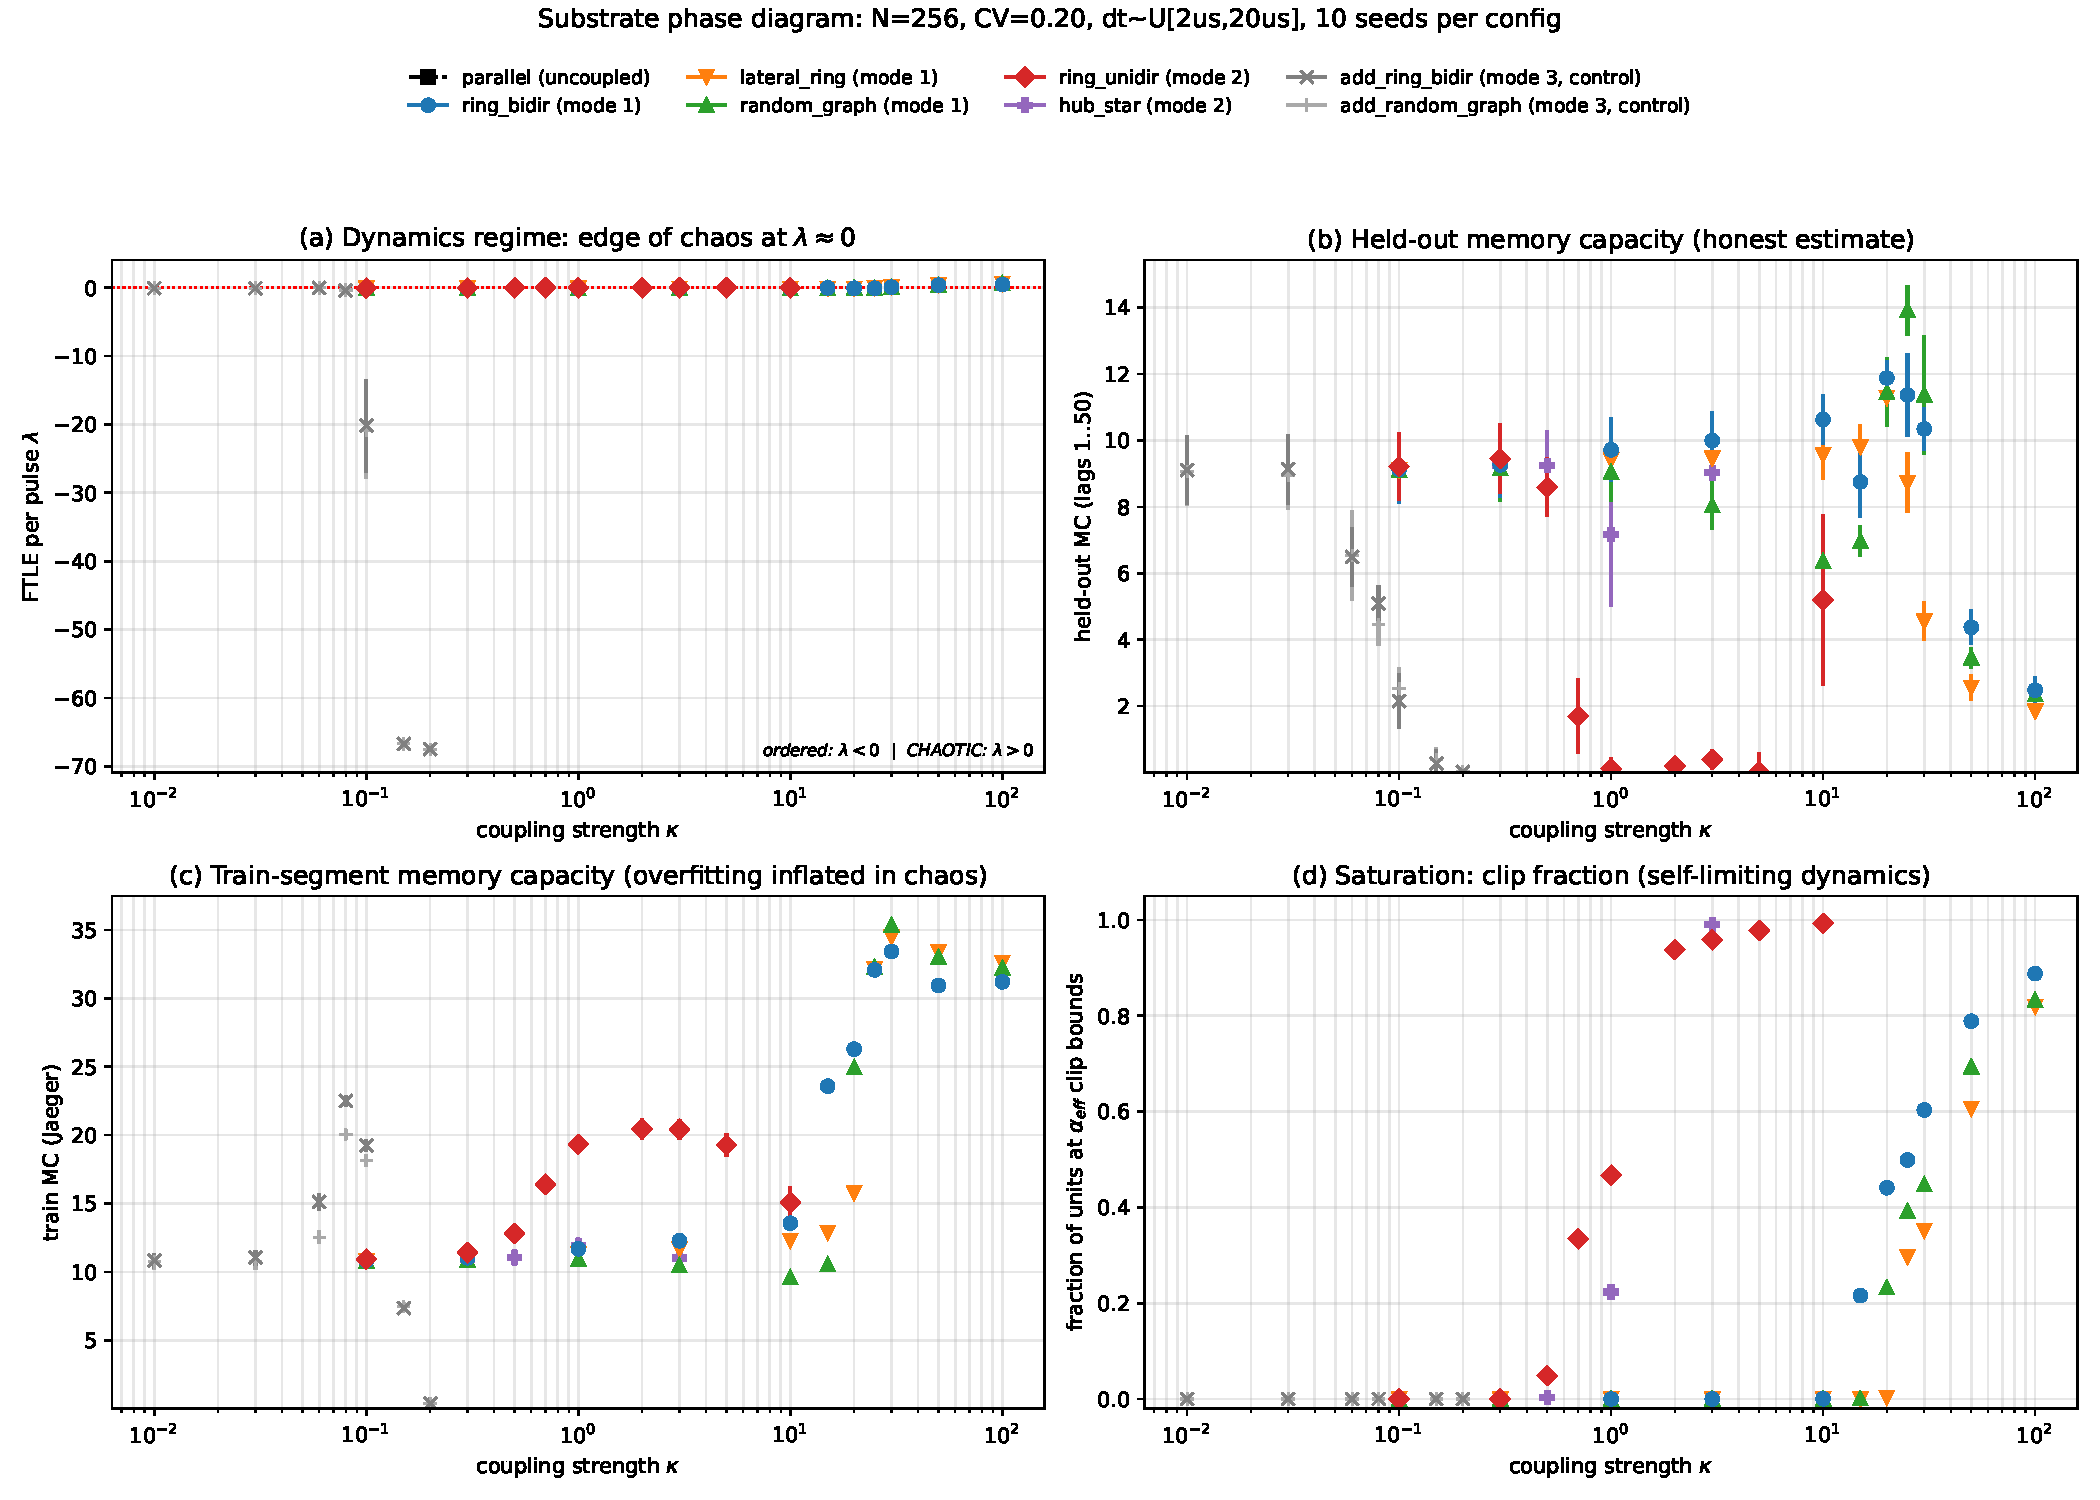
\includegraphics[width=0.92\textwidth]{substrate_phase_diagram_v2}
\caption{Phase diagram (Paper A, Fig.~2): $\kappa$ vs.\ finite-time Lyapunov
exponent, held-out and in-sample MC, and clip fraction across topology
families.}
\label{fig:phasediagram}
\end{figure}

\begin{figure}[t]
\centering
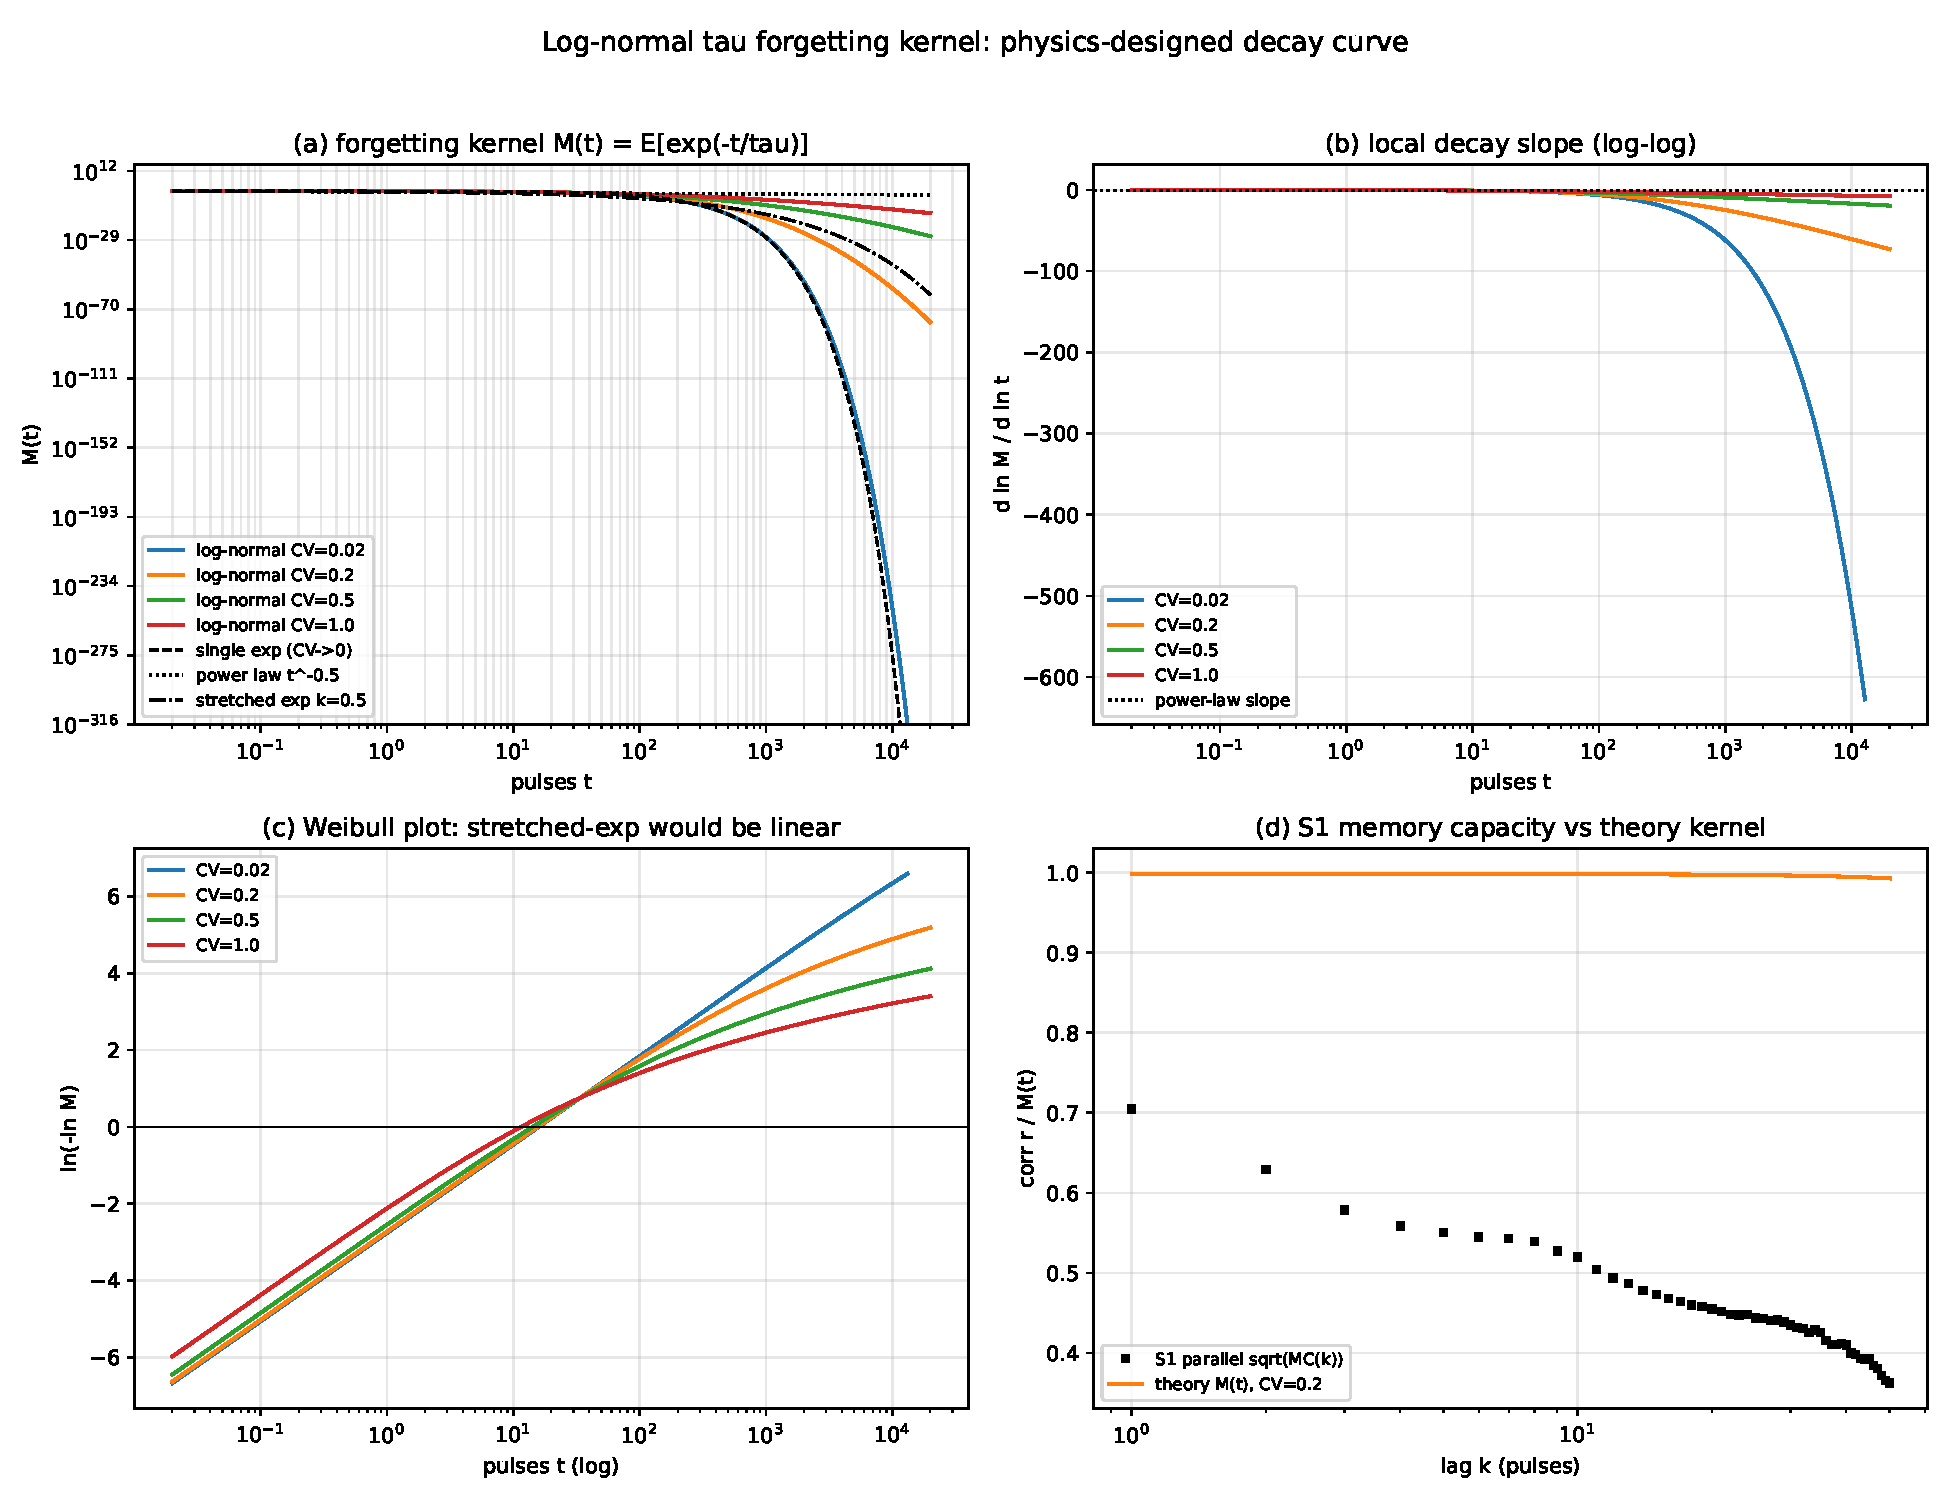
\includegraphics[width=0.92\textwidth]{forgetting_curve_theory}
\caption{Forgetting kernel (Paper A, Fig.~3): $M(t)$ curves over CV, tail
slopes, and the overlay of the measured $\sqrt{\MCI(k)}$ on $M(k\bar{\Dt})$
(Pearson $r=0.97$).}
\label{fig:forgetting}
\end{figure}

\begin{figure}[t]
\centering
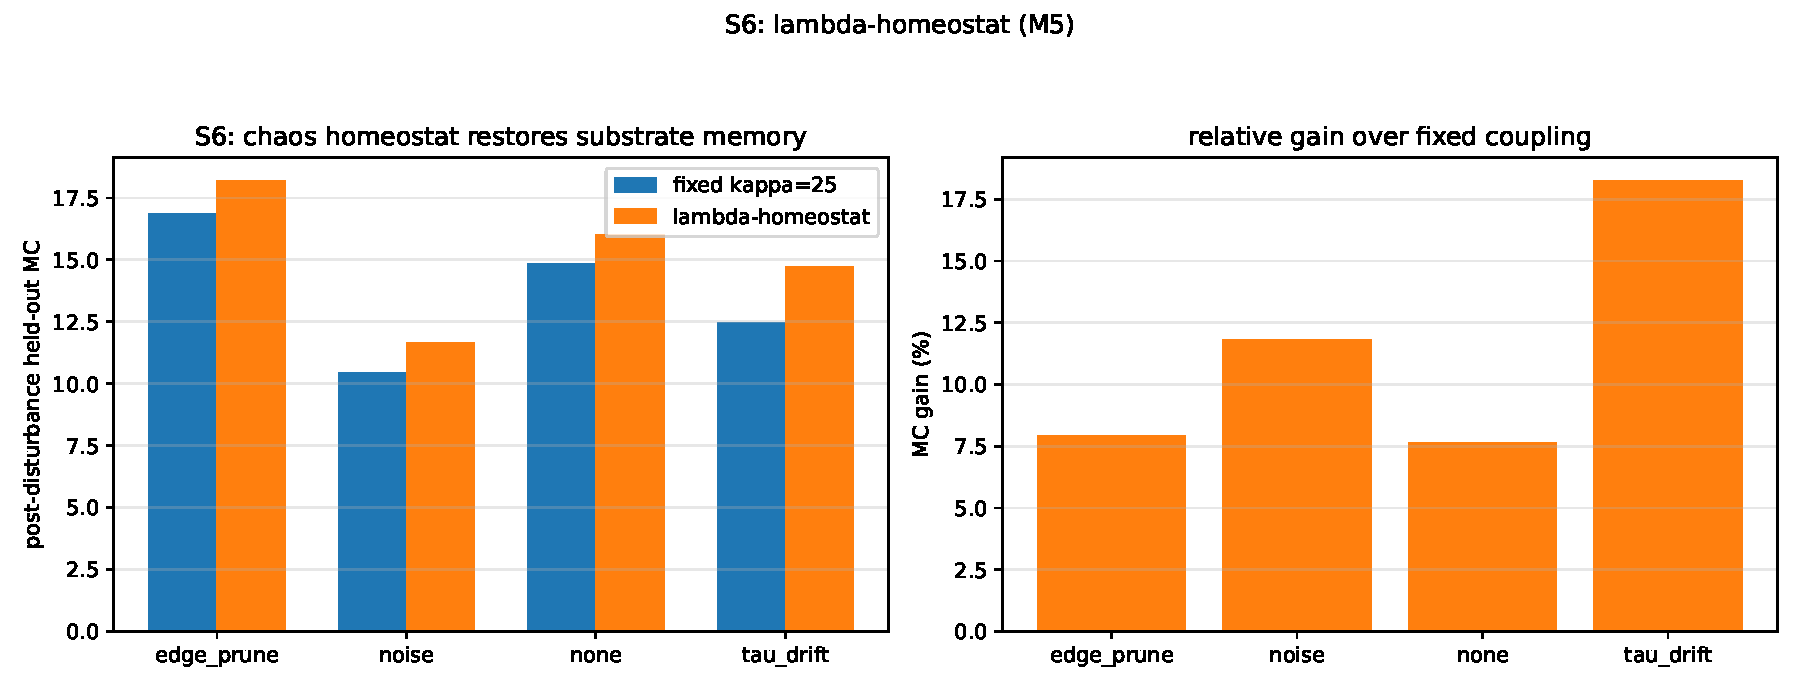
\includegraphics[width=0.75\textwidth]{paperA_fig4_robustness}
\caption{$\lambda$-homeostat robustness (Paper A, Fig.~4): post-disturbance
held-out MC gains over fixed coupling (Table~\ref{tab:homeostat}).}
\label{fig:robustness}
\end{figure}

\appendix
\counterwithin{equation}{section}
\setcounter{equation}{0}

\section{Derivation details}
\label{app:derivations}

\subsection{The trap spectrum is log-normal (Section~\ref{sec:model})}
\label{app:spectrum}

A shallow trap escapes by thermally activated emission with rate
$\nu e^{-E/(kT)}$, so a single trap's time constant is
$\tau(E)=\nu^{-1}e^{E/(kT)}$. With median activation energy $E_a$,
$\tau_0=\nu^{-1}e^{E_a/(kT)}$; for $E_a=0.55$~eV, $\nu=10^{13}$~s$^{-1}$,
$T=300$~K ($kT\approx 25.85$~meV): $\tau_0=10^{-13}e^{0.55/0.02585}\,\text{s}
\approx 174\,\mu$s. If the activation energy varies across devices as
$E_i=E_a+\Delta E_i$ with $\Delta E_i\sim\mathcal{N}(0,\sigma_E^2)$, then
\begin{equation}
\ln\tau_i=\ln\nu^{-1}+(E_a+\Delta E_i)/(kT)\sim\mathcal{N}
\big(\ln\tau_0,\ \sigma_E^2/(kT)^2\big),
\label{eq:spectrum}
\end{equation}
i.e., $\tau_i$ is log-normal with $\sigma^2=\sigma_E^2/(kT)^2$ and
$\mathrm{CV}^2=e^{\sigma^2}-1$. The CV $=0.20$ used throughout corresponds to a
spread $\sigma_E=kT\sqrt{\ln(1+0.20^2)}\approx 5.1$~meV --- a few-meV
fabrication spread --- which motivates treating CV as a physically plausible
design knob rather than a free hyperparameter.

\subsection{Per-pulse update and the order independence of coupling (Section~\ref{sec:model})}
\label{app:update}

Over a write pulse of width $p_w$, the injection term drives occupancy toward 1
at rate $\alpha_{\mathrm{eff},i}$; over the inter-pulse interval $\Dt_t$ both
the injected and the pre-existing occupancy relax with the trap time constant.
The discrete per-pulse map (Eq.~\eqref{eq:update}) is the composition of one
injection step and one relaxation step:
\begin{equation}
x_i(t+1)=\Big[x_i(t)+\alpha_{\mathrm{eff},i}(t)\big(1-x_i(t)\big)\Big]\,
e^{-(p_w+\Dt_t)/\tau_i}.
\label{eq:update2}
\end{equation}
Two-pass order independence: the contrast $g_i(t)$ is evaluated from the
\emph{pre-update} state $x(t)$ alone (neighbor current ratios at time $t$), and
all $N$ units are then updated simultaneously from the same pre-update state.
The map is therefore a well-defined function of the state at $t$ --- a parallel
map --- and the order in which individual unit updates are computed is
irrelevant. At $\kappa=0$, $\alpha_{\mathrm{eff},i}=\alpha_0$ for all $i$ and
the coupling term vanishes; the map reduces exactly to the parallel array of
\cite{prior} (verified to $\le 10^{-10}$ in the implementation's self-test).

\subsection{The forgetting kernel and its quadrature (Section~\ref{sec:kernel})}
\label{app:quadrature}

For a single trap the linear memory of an input at lag $t$ decays as
$e^{-t/\tau}$; averaging over the log-normal spectrum gives
Eq.~\eqref{eq:kernel}. Substituting $z=(\ln\tau-\mu)/(\sqrt{2}\sigma)$, with
$d\tau=\sqrt{2}\,\sigma e^{\mu+\sqrt{2}\sigma z}dz$ and
$p(\tau)d\tau=\pi^{-1/2}e^{-z^2}dz$:
\begin{equation}
M(t)=\pi^{-1/2}\int_{-\infty}^{\infty}e^{-z^2}\exp\!\big(-t\,e^{-(\mu+\sqrt{2}
\sigma z)}\big)\,dz \;\approx\; \pi^{-1/2}\sum_{i=1}^{n} w_i\,\exp\!\big(-t\,e^{-
(\mu+\sqrt{2}\sigma z_i)}\big),
\label{eq:quadrature}
\end{equation}
where $(z_i,w_i)$ are the $n$-point Gauss--Hermite nodes and weights ($n=160$
used; the quadrature is exact to machine precision for $t$ up to $10^4$
pulses).

\textbf{Median pinning of the $1/e$ horizon.} The integrand peaks at
$\tau^*(t)$ where the saddle-point condition
$t/\tau^*=1+(\ln\tau^*-\mu)/\sigma^2$ holds (from
$d/d\tau\,[\ln p(\tau)-t/\tau]=0$). At $t=\tau_0$ the solution is
$\tau^*=\tau_0$ up to a weak CV-dependent correction, so $M(\tau_0)\approx
e^{-1}$: the $1/e$ horizon is pinned at $\approx\tau_0/\bar{\Dt}\approx
16$ pulses regardless of CV (numerically 12--16 pulses for CV
$\in[0.02,1.0]$, Fig.~\ref{fig:forgetting}).

\textbf{Tail asymptotics.} For $t\gg\tau_0$ the saddle point moves to
$\tau^*\approx t\,\sigma^2/\ln(t/\tau_0)$, and
$\ln M(t)\approx-(\ln\tau^*-\mu)^2/(2\sigma^2)-t/\tau^*$; dropping the
$t/\tau^*$ term gives the leading-order log--log slope
\begin{equation}
\frac{d\ln M}{d\ln t}\approx -\frac{\ln t-\mu}{\sigma^2}.
\label{eq:tailslope}
\end{equation}
The $t/\tau^*$ correction is not sub-leading in the sampled window: over
$t\in[5{,}000,\,20{,}000]$ pulses the exact quadrature slope is $-60.6$ at
CV $=0.2$ ($\sigma^2=0.0392$; $\mu=\ln(\tau_0/\bar{\Dt})\approx2.76$ in pulse
units), while Eq.~\eqref{eq:tailslope} gives $-147$ to $-182$ --- the
asymptotic regime is only partially reached (at $t=200$ the exact slope is
already $-9.3$, against the formula's $-64.8$). The qualitative prediction is
confirmed: the slope steepens as the spectrum narrows (quadrature $-60.6$ at
CV $=0.2$ vs.\ $-7.1$ at CV $=1.0$; Eq.~\eqref{eq:tailslope}: $-147$ to
$-182$ vs.\ $-8.3$ to $-10.3$), and CV$\to0$ makes $\sigma^2\to0$ and the
slope $\to-\infty$: the single-exponential limit.

\subsection{Benettin algorithm (Section~\ref{sec:methods})}
\label{app:benettin}

\begin{enumerate}
\item Evolve the main trajectory $x(t)$ under the fixed drive stream for the
full collection window.
\item At each renormalization point $t_m=m\,T_{\mathrm{ren}}$
($T_{\mathrm{ren}}=10$ pulses), create the twin $\tilde{x}(t_m)=x(t_m)+\delta$
with $\delta_i\sim U(-\epsilon,\epsilon)$ per unit, $\epsilon=10^{-8}$.
\item Evolve $\tilde{x}$ in parallel with $x$ under the \emph{identical} drive
sequence for $T_{\mathrm{ren}}$ pulses.
\item Measure the separation
$d_m=\|\tilde{x}(t_{m+1})-x(t_{m+1})\|_2$, accumulate
$\ln(d_m/(\epsilon\sqrt{N}))$, and renormalize the twin onto the reference
direction: $\tilde{x}\leftarrow x+(\epsilon\sqrt{N})(\tilde{x}-x)/d_m$.
\item After $M$ renormalization blocks,
$\lambda\approx(MT_{\mathrm{ren}})^{-1}\sum_{m=1}^{M}\ln(d_m/(\epsilon
\sqrt{N}))$ per pulse.
\end{enumerate}

The estimate is finite-time and resolution-limited near zero
($|\lambda|\lesssim10^{-3}$ is indistinguishable from 0); the perturbation
$\epsilon$ is small enough that the linearized dynamics dominates within one
block.

\subsection{Memory-capacity estimator and the linear-reservoir closed form (Section~\ref{sec:methods})}
\label{app:mc}

For lag $k$ the target is $y_k(t)=\Dt_{t-k}$ and the features are the
standardized current ratios plus bias, $\phi_t$. Ridge regression on the first
70\% of the stream solves $W_k=(\Phi^\top\Phi+\lambda_r I)^{-1}\Phi^\top Y_k$
(targets mean-centered); evaluation is on the last 30\% after a
$k_{\max}=50$-step leakage buffer, so no evaluation target references
training-segment inputs. The per-lag capacity is the squared multiple
correlation $\MCI(k)=r_k^2=\mathrm{corr}(y_k,\hat{y}_k)^2$,
$\MCI_{\mathrm{total}}=\sum_{k=1}^{50}r_k^2$.

\textit{Linear closed form.} Linearize the substrate (clip inactive, $\kappa$
small): $x_{t+1}=A x_t+b u_{t+1}$ with $u_t=\Dt_t$ and $A$ contractive. Then
$x_t=\sum_{j\ge0}A^j b\,u_{t-j}$; the input at lag $k$ contributes the
component $A^{k}b\,u_{t-k}$, whose covariance with $x_t$ is
$c_k=A^{k}b\,\mathrm{Var}(u)$. The best linear predictor achieves the
multiple correlation
\begin{equation}
\MCI(k)=c_k^\top\,\Sigma_x^{-1}\,c_k,\qquad
\Sigma_x=\mathrm{Var}(x_t)=\sum_{j\ge0}A^j bb^\top(A^\top)^j\,\mathrm{Var}(u),
\label{eq:mc}
\end{equation}
and Dambre et al.\ \cite{dambre2012} show the total linear capacity of an
$N$-dimensional linear system is bounded by the state dimension:
$\sum_k \MCI(k)\le N$, with equality attained by orthogonally normalized
dynamics. The measured nonlinear-substrate curve is estimated with the held-out
protocol of Section~\ref{sec:methods}; the closed form anchors the theory at
the linear limit.

\section*{Supplementary Material}
\label{sec:supp}

\textbf{Supplementary Note 1. Task-level CV sweep (Fig.~S1).} At the task level
(held-out MC at the memory-optimal operating points, CV
$\in\{0.1,0.2,0.4\}$, 10 seeds), the uncoupled substrate follows the
single-unit kernel theory: MC rises 2.54 $\to$ 3.37 ($+33\%$) as CV widens from
0.1 to 0.4 --- the heavier tail retains more old lags. The coupled substrate at
the near-critical optimum behaves \emph{oppositely}: random\_graph
$\kappa=25$ MC falls 12.93 $\to$ 7.33 as CV widens (narrow spectrum best), and
ring\_bidir $\kappa=20$ falls 9.55 $\to$ 7.86. The collective near-critical
state prefers homogeneous timescales --- heterogeneous relaxation rates disrupt
the synchronization of the contrast-feedback loop. The CV knob's direction
therefore depends on the operating regime: wide spectra for parallel
(kernel-dominated) operation, narrow spectra for coupled near-critical
operation.

\begin{figure}[t]
\centering
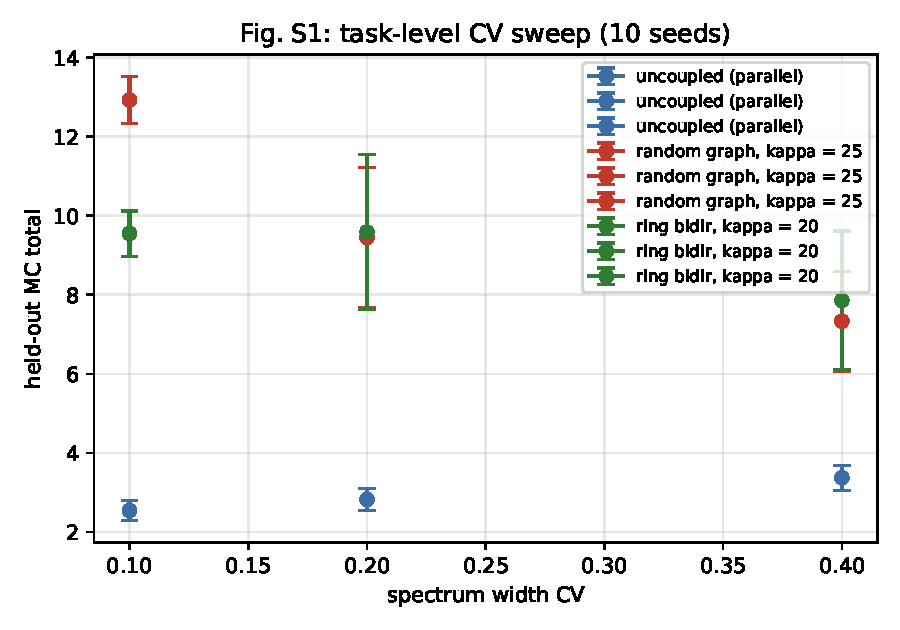
\includegraphics[width=0.6\textwidth]{paperA_figS1_cv_sweep}
\caption{Supplementary Fig.~S1: task-level CV sweep (held-out MC vs.\ CV, 10
seeds; data/s10\_cv\_sweep\_v1.csv).}
\label{fig:supp1}
\end{figure}

\section*{Declaration of competing interest}

The author declares no known competing financial interests or personal
relationships that could have appeared to influence the work reported in
this paper.

\section*{Funding}

This research did not receive any specific grant from funding agencies in
the public, commercial, or not-for-profit sectors.

\section*{Code and data availability}

All simulation scripts and generated data are available at
\url{https://github.com/huyamingc/REDEM} (private during review; released on
acceptance).

\begin{thebibliography}{12}

\bibitem{maass2002} Maass, W., Natschläger, T. \& Markram, H. Real-time
computing without stable states: a new framework for neural computation based
on perturbations. \emph{Neural Computation} \textbf{14}(11), 2531--2560 (2002).
\url{https://doi.org/10.1162/089976602760407955}

\bibitem{larger2012} Larger, L. \emph{et al.} Photonic information processing
beyond Turing: an optoelectronic implementation of reservoir computing.
\emph{Opt.~Express} \textbf{20}, 3241--3249 (2012).

\bibitem{du2017} Du, C., Cai, F., Zidan, M. A., Ma, W., Lee, S. H. \& Lu, W. D.
Reservoir computing using dynamic memristors for temporal information
processing. \emph{Nature Communications} \textbf{8}, 2204 (2017).

\bibitem{prior} Hu, Y. Si$_3$N$_4$ shallow-trap relaxation for temporal
pattern encoding: a systematic design-space analysis. Zenodo preprint,
\url{https://doi.org/10.5281/zenodo.21753791} (2026); substrate
calibration source for this work.

\bibitem{jaeger2001} Jaeger, H. The ``echo state'' approach to analysing and
training recurrent neural networks. GMD Report 148 (2001).
\url{https://www.ai.rug.nl/minds/uploads/EchoStatesTechRep.pdf}

\bibitem{bertschinger2004} Bertschinger, N. \& Natschläger, T. Real-time
computation at the edge of chaos in recurrent neural networks.
\emph{Neural Computation} \textbf{16}(7), 1413--1436 (2004).
\url{https://doi.org/10.1162/089976604323057443}

\bibitem{dambre2012} Dambre, J., Verstraeten, D., Schrauwen, B. \& Massar, S.
Information processing capacity of dynamical systems.
\emph{Scientific Reports} \textbf{2}, 514 (2012).

\bibitem{fusi2005} Fusi, S., Drew, P. J. \& Abbott, L. F. Cascade models of
synaptically stored memories. \emph{Neuron} \textbf{46}(4), 599--609 (2005).

\bibitem{benna2016} Benna, M. K. \& Fusi, S. Computational principles of
synaptic memory consolidation. \emph{Nature Neuroscience} \textbf{19}(12),
1697--1706 (2016). \url{https://doi.org/10.1038/nn.4401}

\bibitem{boyd1985} Boyd, S. \& Chua, L. O. Fading memory and the problem of
approximating nonlinear operators with Volterra series.
\emph{IEEE Trans.\ Circuits Syst.} \textbf{32}(11), 1151--1161 (1985).

\bibitem{pathak2018} Pathak, J., Hunt, B., Girvan, M., Lu, Z. \& Ott, E.
Model-free prediction of large spatiotemporally chaotic systems from data: a
reservoir computing approach. \emph{Phys.\ Rev.\ Lett.} \textbf{120}, 024102
(2018). \url{https://doi.org/10.1103/PhysRevLett.120.024102}

\bibitem{companionB} Author's companion Paper B: REDEM: Online Learning
with Meta-Adaptation and Structural Plasticity for Non-Stationary
Environments (online learning architecture),
\emph{companion preprint} (2026),
\url{https://doi.org/10.5281/zenodo.22110607}.

\end{thebibliography}

\end{document}
